%\documentclass
\documentclass{article}

\usepackage{titlesec}
\usepackage{graphicx}
\usepackage{subcaption}
\usepackage{wrapfig}
\usepackage{caption}
\usepackage[
backend=biber,
style=alphabetic,
sorting=ynt
]{biblatex}

\usepackage{multirow}

\addbibresource{bibliography.bib} 

\titleformat{\section}[block]{\filcenter\Large\bfseries}{}{1em}{}
\captionsetup[figure]{labelformat=empty}

\title{Vynil Revival: El renacer del formato del vinilo en el siglo XXI}
\author{Ivan Dario Gonzalez Collazos}
\date{Mayo 31 del 2023}

\begin{document}

\maketitle

\section{¿Qué paso con el vinilo?}

\begingroup
\setlength{\intextsep}{0pt}%
\setlength{\columnsep}{0pt}%

\begin{wrapfigure}{r}{0.55\textwidth}
    \centering
    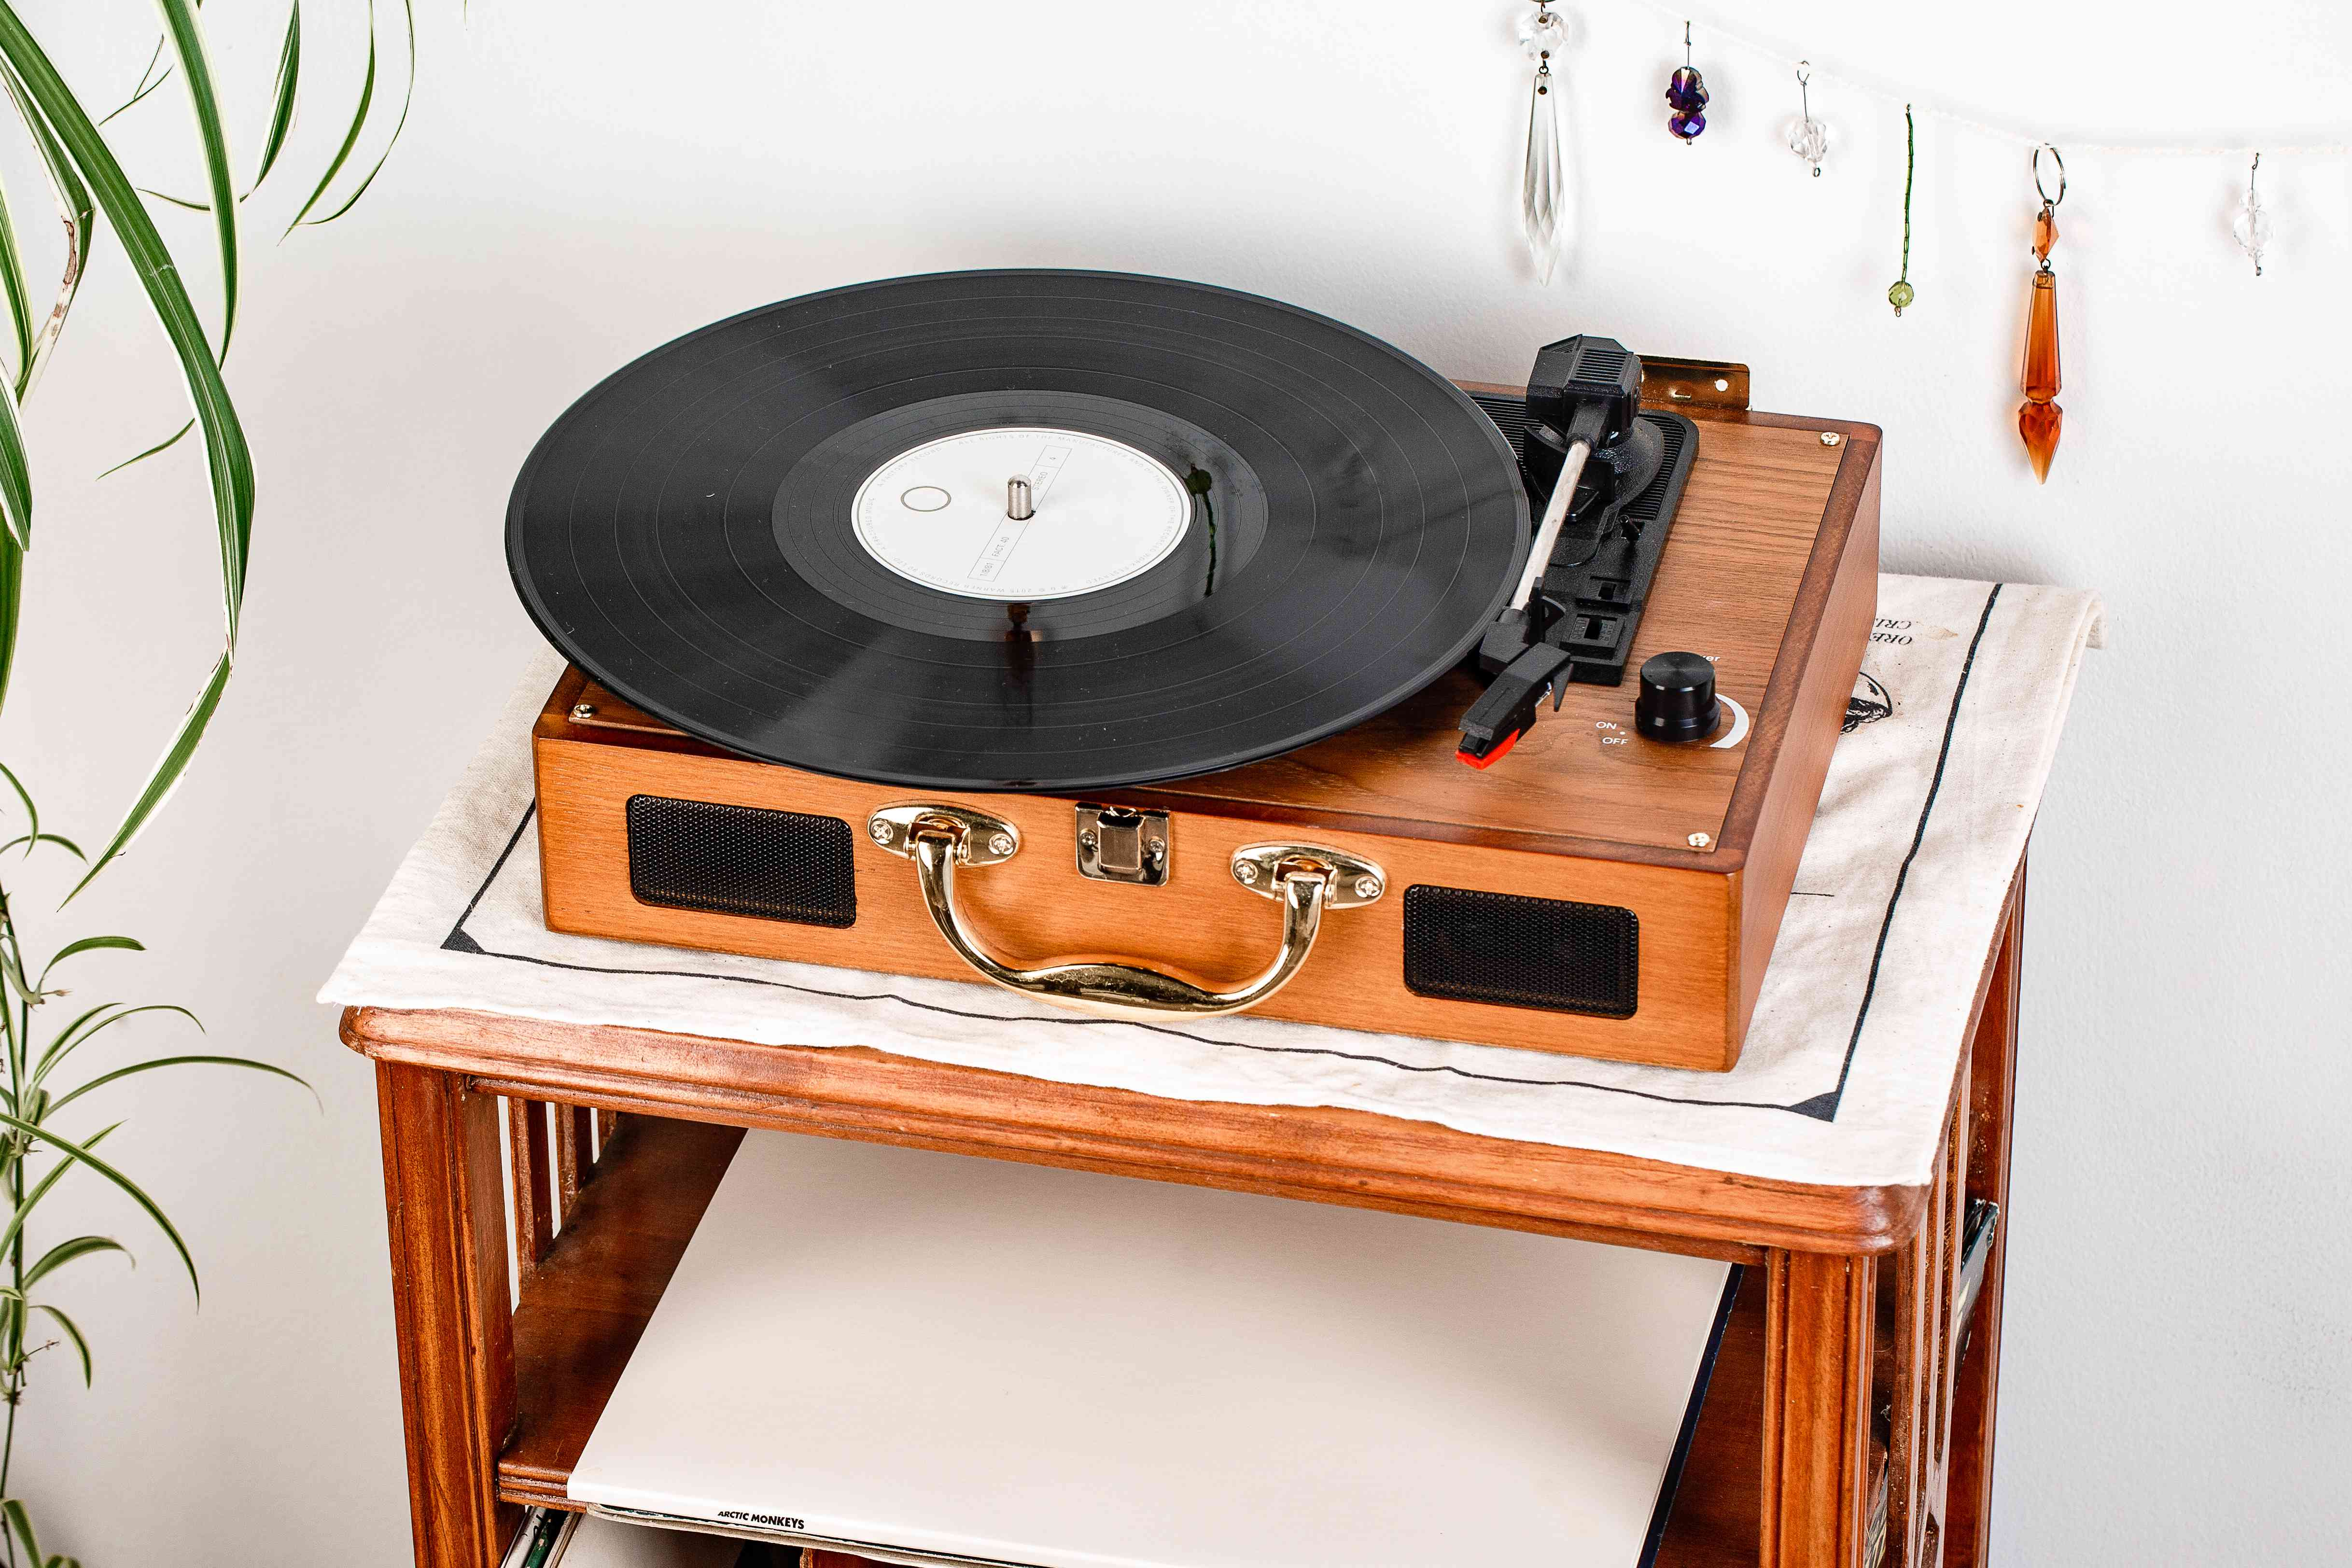
\includegraphics[width=0.45\textwidth]{images/vynil.jpg}
    \vspace{-5pt}
    \caption{LP o Vinilo}
\end{wrapfigure}

Desde su invención al final de la década de 1940, el formato LP (O vinilo) fue uno de los métodos mas populares para comercializar música durante más de dos décadas, llegando a ser el formato más popular al final de la década de 1970. Sobre el año de 1978 alcanzaría el pico de ventas (en Estados Unidos) llegando a vender más de 300 millones de copias donde empezaría su declive en ventas.\cite{wikirevival}\\

\endgroup

\begingroup
\setlength{\intextsep}{0pt}%
\setlength{\columnsep}{0pt}%

\begin{wrapfigure}{l}{0.55\textwidth}
    \centering
    
\includegraphics[width=0.45\textwidth]{images/cd.jpg}
    \vspace{-5pt}
    \caption{Compact Disk (CD)}
\end{wrapfigure}

Philips lanzaría en 1982 el compact disk (CD), el cual generaría que la industria musical empezara a utilizar este nuevo formato debido a los costos de producción y la comercialización de este en las tiendas. Este avance generaría que el mercado empezara a depreciar el LP y provocaría que los fabricantes abarataran costos donde los discos empezaran a bajar su peso de 180 gramos a 70 y algunos de 50 gramos, siendo fabricados de materiales reciclados y con esto, bajando la calidad.\cite{youtube}\\

\endgroup

Las disqueras empezarían a cerrar las fábricas de vinilos hacia mediados de la década de 1980, empezando el letargo que llevaría a que el LP fuera un artículo de nicho y con un mercado demasiado limitado, llegando a tener durante la década de 1990 e inicios del siglo XXI ventas de un 1 millón de ejemplares por año, siendo el año 2006 el menor de los años vendiendo menos del millón.\cite{wikirevival}\\

\begin{figure}[h]
    \centering
    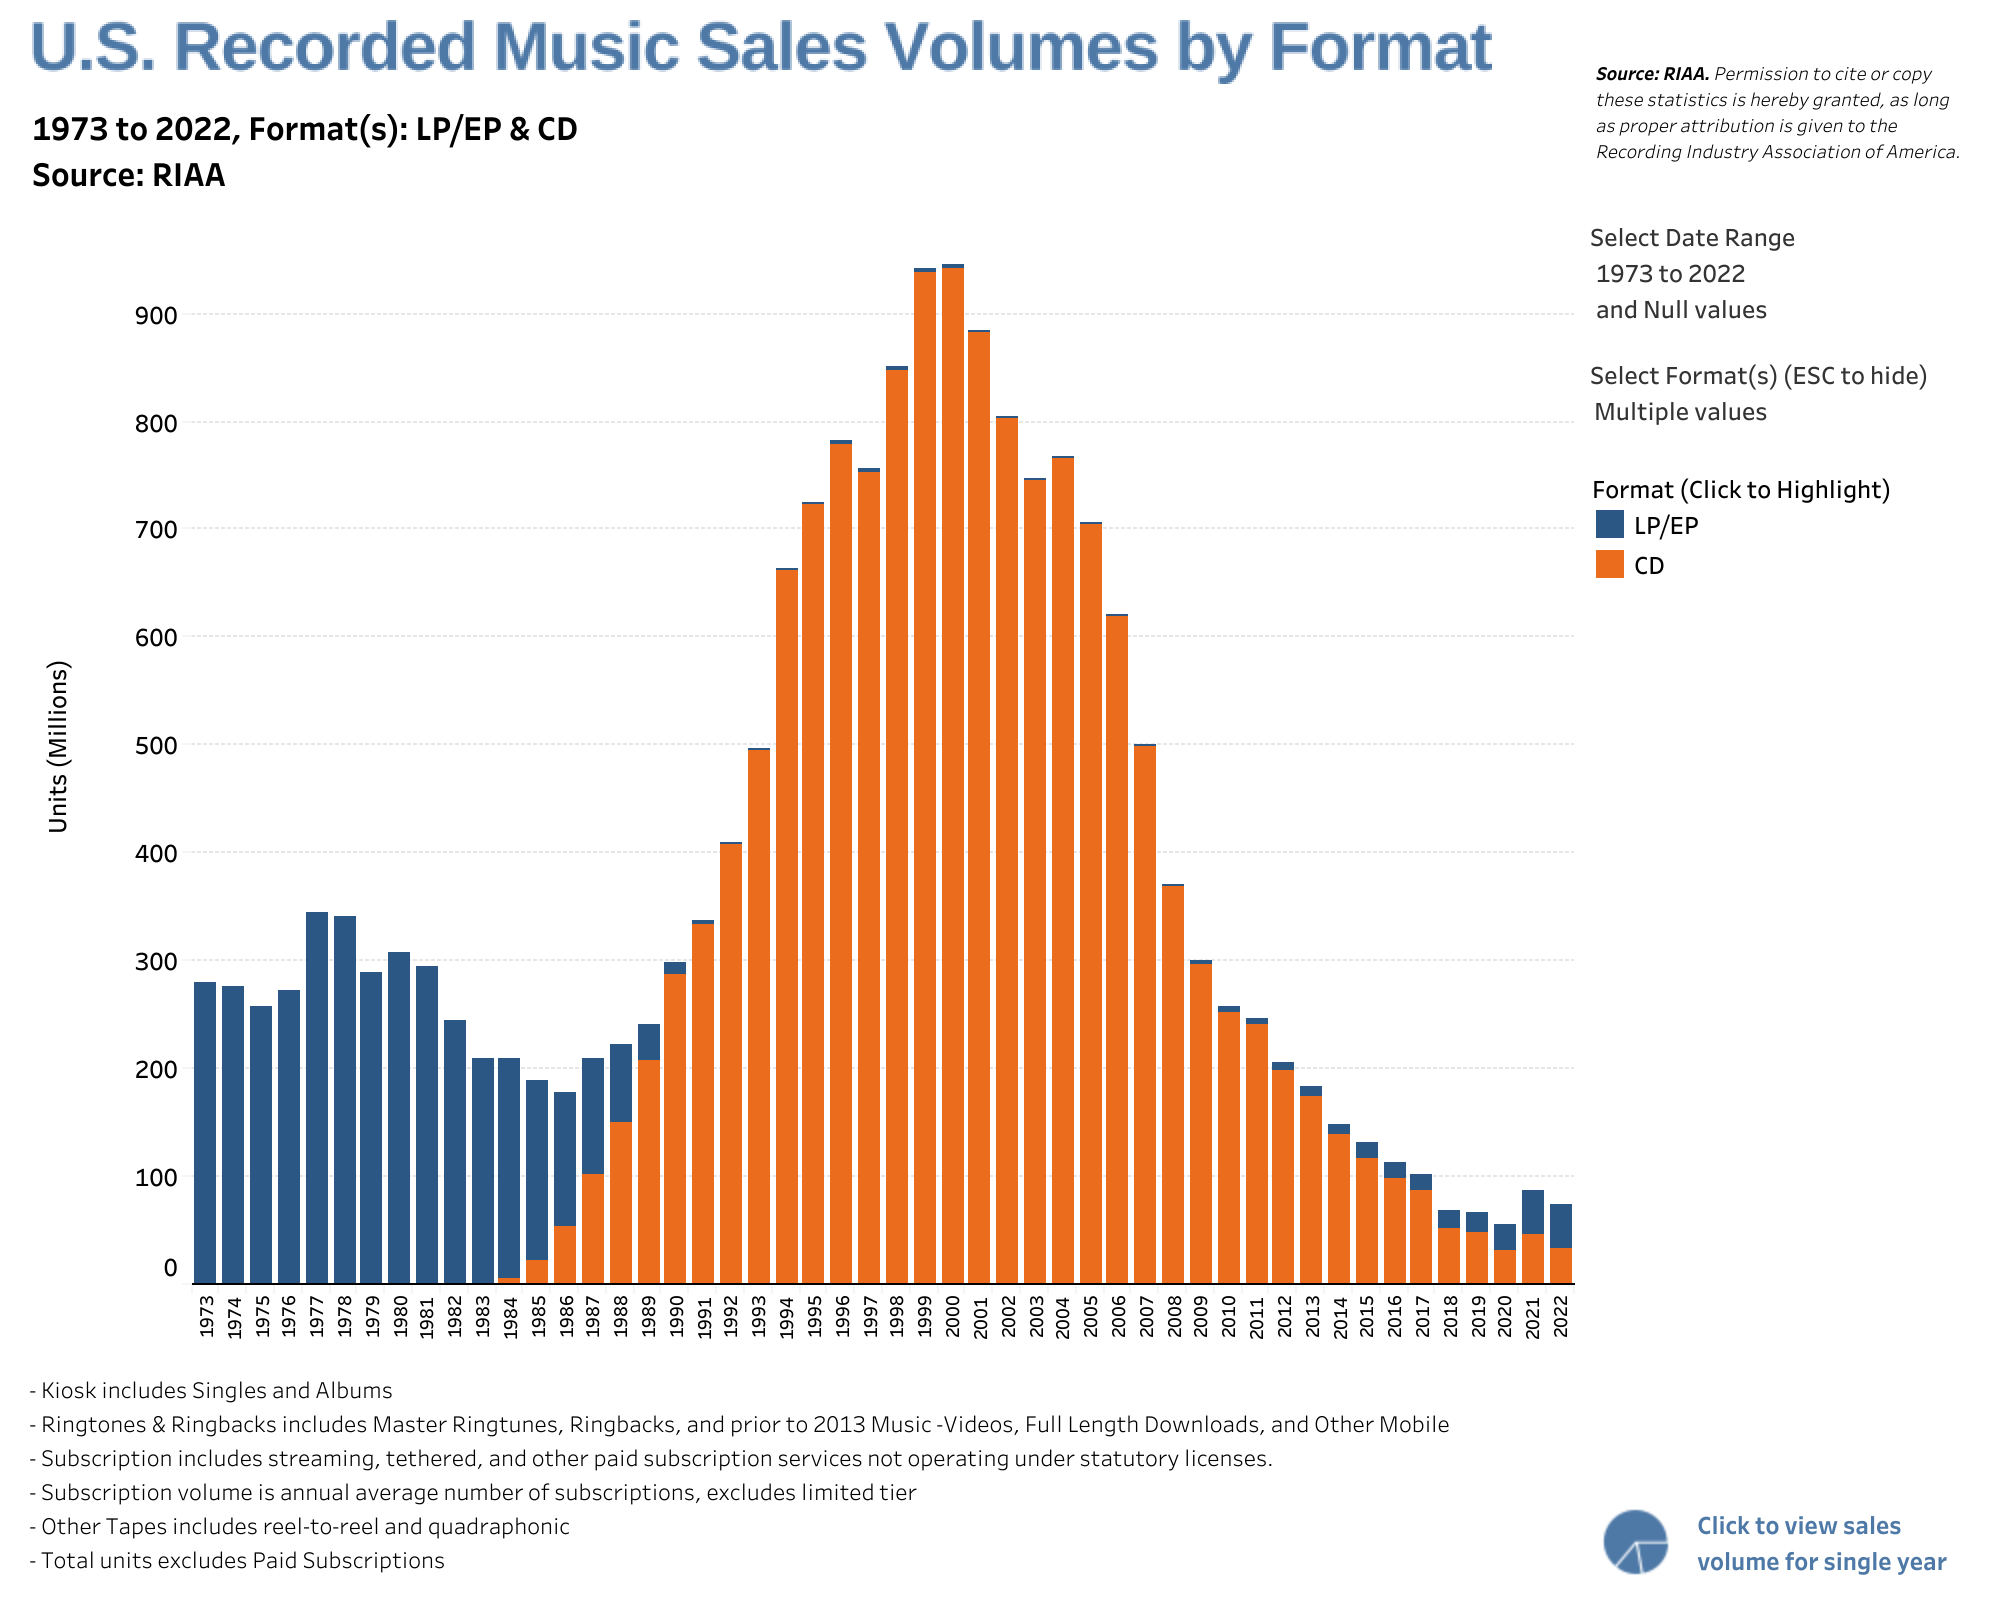
\includegraphics[width=\textwidth]{images/sales.png}
    \vspace{-5pt}
    \caption{Número de unidades vendidas por año del LP y CD.\cite{riaa}}
\end{figure}

En el siglo XXI, surgieron otros medios de difusión de la música, las descargas digitales y las suscripciones a plataformas de streaming, lo cual hizo que los formatos físicos se volvieran mucho mas de nicho, afectando al CD y al LP por igual, donde las ventas de CD empezaron a disminuir desde el 2001 cuando Apple lanza el iPod y revoluciona la manera en la cual se escucha la música.

\section{El vinilo revive}

El fenómeno de la música digital generaría que tiendas de discos cerraran sus puertas o en el mejor de los casos, se redujeran a pequeñas tiendas de nicho para para melómanos y audiófilos aficionados a los formatos físicos.\\

Durante la segunda mitad de la década de los 2000, las ventas de vinilos empezarían a crecer después del 2006, su peor año en ventas, en parte gracias a que personas de todas las edades empezaron a buscar su música favorita en formato físico, lo cual incremento las ventas no solo de los LP sino de agujas, tornamesas y demás equipo que se necesita para poder escuchar música en vinilos en ambientes de alta calidad.\cite{youtube}\\

Acompañado del fenómeno asociado a los aficionados del vinilo, en el 2007 empezó en Record Store Day, una iniciativa creada por las tiendas independiente de discos de la región de Baltimore, Maryland, donde los dueños de tiendas (Eric Levin, Michael Kurtz, Carrie Colliton, Amy Dorfman, Brian Poehner y Don Van Cleave) celebraron en ese año la cultura de las tiendas independientes de discos.\cite{wikiRSD}\\

\begingroup
\setlength{\intextsep}{0pt}%
\setlength{\columnsep}{0pt}%

\begin{wrapfigure}{l}{0.4\textwidth}
    \centering
    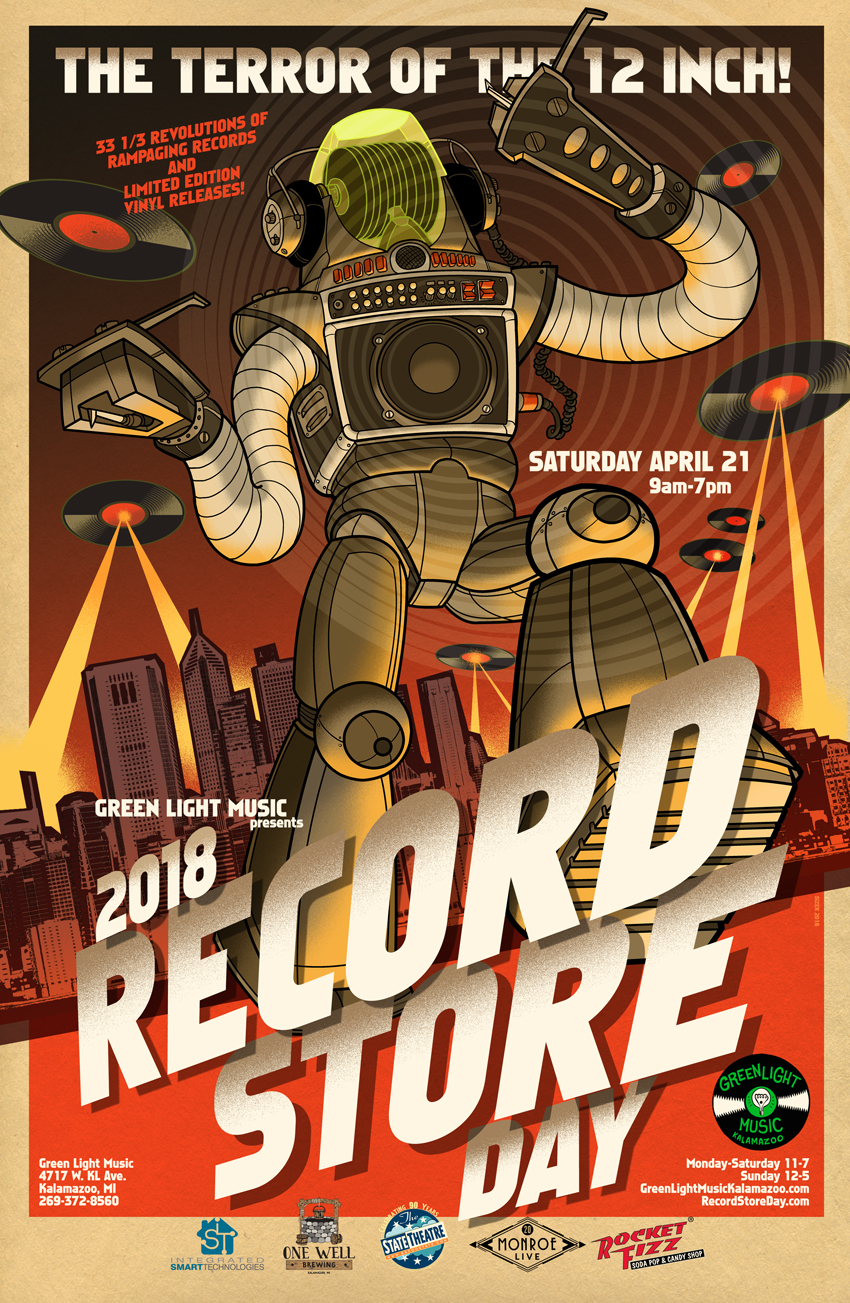
\includegraphics[width=0.3\textwidth]{images/recordday.jpg}
    \vspace{-5pt}
    \caption{Poster del Record Store Day}
\end{wrapfigure}

Los Record Store Day se empezaron a celebrar de una a dos veces al año alrededor del mundo, teniendo apoyo de artistas y bandas mundialmente reconocidas, así como lanzamientos exclusivos de álbumes de bandas independientes como de versiones especiales de discos de bandas ya famosas. Desde el 2008 se celebran estos días generalmente el tercer sábado de abril y en el viernes Negro en noviembre, que reúnen a melómanos, audiófilos y fanáticos del vinilo en torno a un día que celebra a las tiendas de discos, pero que también celebra un formato que se creía extinto.\cite{wikiRSD}\\

\endgroup

Otro factor que permitió el renacimiento del formato LP, fue que las bandas independientes empezaron a prensar sus lanzamientos discográficos, permitiendo que sus fans pudieran tener una copia física de sus álbumes, lo que además de tener su música en streaming les genera ganancias por las ventas de estos.\cite{youtube}\\

Pero el efecto no solo se dio en Estados Unidos, sino también en otros países.\\

\begingroup
\setlength{\intextsep}{0pt}%
\setlength{\columnsep}{0pt}%

\begin{wrapfigure}{r}{0.55\textwidth}
    \centering
    
\includegraphics[width=0.45\textwidth]{images/german.jpg}
    \vspace{-5pt}
    \caption{Escena Rave Alemana}
\end{wrapfigure}

En Alemania, hubo dos momentos donde el vinilo tuvo relevancia; el primero a mediados de la década de 1990, donde la escena rave del país estaba tomando fuerza ya que para los DJs del momento era mejor para mezclar. Además, debido al tamaño de las portadas de los LP, artistas preferían trabajar en esas dimensiones que en las del CD, llevando a un primer renacer en el país europeo. Pero el movimiento decayó al principio de la primera década del siglo XXI, para resucitar en el 2007 con el movimiento a nivel mundial.\cite{wikirevival}\\

\endgroup

En Japón y Reino Unido, la venta de vinilos subió desde 2007, donde bandas locales japonesas empezaron a apoyar a las tiendas de discos con lanzamientos en LP permitiendo que las tiendas subsistieran y pudieran unirse al Record Store Day, además de otros días adicionales inventados por las tiendas japonesas; En Reino Unido, BBC Radio 6 empieza a apoyar el renacimiento del vinilo en 2011, dándole oportunidad a músicos de mostrar y tocar discos de su colección.\cite{wikirevival}

\begin{table}[h]
    \centering
    \scalebox{0.8}{
    \begin{tabular}{|lccc|}
    \hline
    \multicolumn{4}{|c|}{LP mas vendidos desde 2008 en USA}                                                                                                                                                  \\ \hline
    \multicolumn{1}{|c|}{Año}  & \multicolumn{1}{c|}{Disco}                                       & \multicolumn{1}{c|}{Artista}        & \begin{tabular}[c]{@{}c@{}}\# de unidades \\ vendidas\end{tabular} \\ \hline
    \multicolumn{1}{|l|}{2008} & \multicolumn{1}{c|}{In Rainbows}                                 & \multicolumn{1}{c|}{Radiohead}      & 25.800                                                             \\ \hline
    \multicolumn{1}{|l|}{2009} & \multicolumn{1}{c|}{Abbey Road}                                  & \multicolumn{1}{c|}{The Beatles}    & 34.800                                                             \\ \hline
    \multicolumn{1}{|l|}{2010} & \multicolumn{1}{c|}{Abbey Road}                                  & \multicolumn{1}{c|}{The Beatles}    & 35.000                                                             \\ \hline
    \multicolumn{1}{|l|}{2011} & \multicolumn{1}{c|}{Abbey Road}                                  & \multicolumn{1}{c|}{The Beatles}    & 41.000                                                             \\ \hline
    \multicolumn{1}{|l|}{2012} & \multicolumn{1}{c|}{Blunderbuss}                                 & \multicolumn{1}{c|}{Jack White}     & 34.000                                                             \\ \hline
    \multicolumn{1}{|l|}{2013} & \multicolumn{1}{c|}{Random Access Memories}                      & \multicolumn{1}{c|}{Daft Punk}      & 49.000                                                             \\ \hline
    \multicolumn{1}{|l|}{2014} & \multicolumn{1}{c|}{Lazaretto}                                   & \multicolumn{1}{c|}{Jack While}     & 87.000                                                             \\ \hline
    \multicolumn{1}{|l|}{2015} & \multicolumn{1}{c|}{25}                                          & \multicolumn{1}{c|}{Adele}          & 116.000                                                            \\ \hline
    \multicolumn{1}{|l|}{2016} & \multicolumn{1}{c|}{Blackstar}                                   & \multicolumn{1}{c|}{David Bowie}    & 54.000                                                             \\ \hline
    \multicolumn{1}{|l|}{2017} & \multicolumn{1}{c|}{Sgt. Pepper's Lonely Hearts Club Band}       & \multicolumn{1}{c|}{The Beatles}    & 72.000                                                             \\ \hline
    \multicolumn{1}{|l|}{2018} & \multicolumn{1}{c|}{Guardians of the Galaxy: Awesome Mix Vol. 1} & \multicolumn{1}{c|}{Various Artist} & 84.000                                                             \\ \hline
    \multicolumn{1}{|l|}{2019} & \multicolumn{1}{c|}{Abbey Road}                                  & \multicolumn{1}{c|}{The Beatles}    & 246.000                                                            \\ \hline
    \multicolumn{1}{|l|}{2020} & \multicolumn{1}{c|}{Fine Line}                                   & \multicolumn{1}{c|}{Harry Styles}   & 232.000                                                            \\ \hline
    \multicolumn{1}{|l|}{2021} & \multicolumn{1}{c|}{30}                                          & \multicolumn{1}{c|}{Adele}          & 318.000                                                            \\ \hline
    \multicolumn{1}{|l|}{2022} & \multicolumn{1}{c|}{Midnights}                                   & \multicolumn{1}{c|}{Taylor Swift}   & 945.000                                                            \\ \hline
    \end{tabular}}
    \end{table}

    Ahora, artistas y bandas alrededor del mundo están haciendo lanzamientos cada vez más grandes de sus álbumes en formato de vinilo, incluyendo versiones especiales, boxsets, artes y colores alternativos, lo que hace que sean más apetecidos entre sus fans. Artistas como Taylor Swift, Adele y Harry Styles han vendido más de 2 millones de LP ellos solos solo en Estados Unidos, lo que ha permitido que el formato sea viable para las bandas, disqueras, distribuidoras y tiendas.\cite{hustle}\cite{wikirevival}

\section{El mañana}

\begingroup
\setlength{\intextsep}{0pt}%
\setlength{\columnsep}{0pt}%

\begin{wrapfigure}{l}{0.55\textwidth}
    \centering
    
\includegraphics[width=0.45\textwidth]{images/factory.jpg}
    \vspace{-5pt}
    \caption{Fabrica de LPs}
\end{wrapfigure}

Ahora, el vinilo como formato al día de hoy, debe afrontar una cadena de suministro mucho más demandante para hacer LP de calidad de muchas bandas en muchos colores y hasta formas, lo cual hace que las pocas prensadoras que están activas tengan retrasos en sus entregas y no logren cumplir las expectativas de numero de vinilos listos para distribuir. Aunque nuevas fábricas están abriendo en el mundo, es difícil cubrir la demanda y esto puede afectar el renacer. También se tiene que agregar el costo del PVC (materia prima del LP), el cual ha ido incrementando acorde con la demanda que ha generado el renacer del vinilo.\cite{hustle}\\

\endgroup

Pero no todo es malo, en 2022 el LP supero en ventas y unidades vendidas al CD, lo cual hace que el formato sea más popular y se estima que el vinilo siga superando al CD en ventas durante los próximos años. Aunque aún fuera de sus años de gloria, el LP vendió más de 40 millones de unidades en el 2022, siendo una cifra que no se ve desde la década de 1980, permitiendo que la industria recupere un formato físico amado por muchos.\\

\printbibliography[
title={Bibliografía}
]

\end{document}